\documentclass[xcolor=svgnames, 12pt]{beamer}
\usetheme{Madrid}
\usepackage{hyperref}
\usepackage{listings}
\usepackage{tikz}
\usepackage{tikz-timing}[2009/05/15]
\usetikzlibrary{positioning,shapes,shadows,arrows}
\usetikzlibrary{trees}

\usepackage{xxcolor}
\usetikzlibrary{chains,matrix,scopes,decorations.shapes,arrows,shapes}


\newcounter{wavenum}

\setlength{\unitlength}{1cm}
% advance clock one cycle, not to be called directly
\newcommand*{\clki}{
  \draw (t_cur) -- ++(0,.3) -- ++(.5,0) -- ++(0,-.6) -- ++(.5,0) -- ++(0,.3)
    node[time] (t_cur) {};
}

\newcommand*{\bitvector}[3]{
  \draw[fill=#3] (t_cur) -- ++( .1, .3) -- ++(#2-.2,0) -- ++(.1, -.3)
                         -- ++(-.1,-.3) -- ++(.2-#2,0) -- cycle;
  \path (t_cur) -- node[anchor=mid] {#1} ++(#2,0) node[time] (t_cur) {};
}

% \known{val}{length}
\newcommand*{\known}[2]{
    \bitvector{#1}{#2}{white}
}

% \unknown{length}
\newcommand*{\unknown}[2][XXX]{
    \bitvector{#1}{#2}{black!20}
}

% \bit{1 or 0}{length}
\newcommand*{\bit}[2]{
  \draw (t_cur) -- ++(0,.6*#1-.3) -- ++(#2,0) -- ++(0,.3-.6*#1)
    node[time] (t_cur) {};
}

% \unknownbit{length}
\newcommand*{\unknownbit}[1]{
  \draw[ultra thick,black!50] (t_cur) -- ++(#1,0) node[time] (t_cur) {};
}

% \nextwave{name}
\newcommand{\nextwave}[1]{
  \path (0,\value{wavenum}) node[left] {#1} node[time] (t_cur) {};
  \addtocounter{wavenum}{-1}
}

% \clk{name}{period}
\newcommand{\clk}[2]{
    \nextwave{#1}
    \FPeval{\res}{(\wavewidth+1)/#2}
    \FPeval{\reshalf}{#2/2}
    \foreach \t in {1,2,...,\res}{
        \bit{\reshalf}{1}
        \bit{\reshalf}{0}
    }
}

% \begin{wave}[clkname]{num_waves}{clock_cycles}
\newenvironment{wave}[3][clk]{
  \begin{tikzpicture}[draw=black, yscale=.7,xscale=1]
    \tikzstyle{time}=[coordinate]
    \setlength{\unitlength}{1cm}
    \def\wavewidth{#3}
    \setcounter{wavenum}{0}
    \nextwave{#1}
    \foreach \t in {0,1,...,\wavewidth}{
      \draw[dotted] (t_cur) +(0,.5) node[above] {t=\t} -- ++(0,.4-#2);
      \clki
    }
}{\end{tikzpicture}}

\tikzset{
  nonterminal/.style={
    % The shape:
    rectangle,
    % The size:
    minimum size=6mm,
    % The border:
    very thick,
    draw=red!50!black!50,         % 50% red and 50% black,
                                  % and that mixed with 50% white
    % The filling:
    top color=white,              % a shading that is white at the top...
    bottom color=red!50!black!20, % and something else at the bottom
    % Font
    font=\itshape
  },
  terminal/.style={
    % The shape:
    rounded rectangle,
    minimum size=6mm,
    % The rest
    very thick,draw=black!50,
    top color=white,bottom color=black!20,
    font=\ttfamily},
  skip loop/.style={to path={-- ++(0,#1) -| (\tikztotarget)}}
}
{
  \tikzset{terminal/.append style={text height=1.5ex,text depth=.25ex}}
  \tikzset{nonterminal/.append style={text height=1.5ex,text depth=.25ex}}
}


\renewcommand\familydefault{\sfdefault}


% Defines a `datastore' shape for use in DFDs.  This inherits from a
% rectangle and only draws two horizontal lines.
\makeatletter
\pgfdeclareshape{datastore}{
  \inheritsavedanchors[from=rectangle]
  \inheritanchorborder[from=rectangle]
  \inheritanchor[from=rectangle]{center}
  \inheritanchor[from=rectangle]{base}
  \inheritanchor[from=rectangle]{north}
  \inheritanchor[from=rectangle]{north east}
  \inheritanchor[from=rectangle]{east}
  \inheritanchor[from=rectangle]{south east}
  \inheritanchor[from=rectangle]{south}
  \inheritanchor[from=rectangle]{south west}
  \inheritanchor[from=rectangle]{west}
  \inheritanchor[from=rectangle]{north west}
  \backgroundpath{
    %  store lower right in xa/ya and upper right in xb/yb
    \southwest \pgf@xa=\pgf@x \pgf@ya=\pgf@y
    \northeast \pgf@xb=\pgf@x \pgf@yb=\pgf@y
    \pgfpathmoveto{\pgfpoint{\pgf@xa}{\pgf@ya}}
    \pgfpathlineto{\pgfpoint{\pgf@xb}{\pgf@ya}}
    \pgfpathmoveto{\pgfpoint{\pgf@xa}{\pgf@yb}}
    \pgfpathlineto{\pgfpoint{\pgf@xb}{\pgf@yb}}
 }
}
\makeatother

%\newcommand{\alice}[1]{\todo[color=green!40]{#1}}
%\newcommand{\bob}[1]{\todo[color=purple!40]{#1}}
\def\degr{${}^\circ$}

\newif\ifcomment
\definecolor{UCLABlue}{RGB}{83, 104, 149}
\definecolor{UCLAGold}{RGB}{254, 187, 54}
\definecolor{bgblue}{rgb}{0.41961,0.80784,0.80784}%
\definecolor{bgred}{rgb}{1,0.61569,0.61569}%
\definecolor{fgblue}{rgb}{0,0,0.6}%
\definecolor{fgred}{rgb}{0.6,0,0}%

\usecolortheme[named=UCLABlue]{structure}
\setbeamertemplate{navigation symbols}{}
\author[P. Tracton]{Philip Tracton}

\institute[UCLA Extension]{
UCLA Extension\\
Department of Engineering and Technology\\
Los Angeles, CA 91340\\
}
\date{\today}

\title[Experimental]{Experimental}

\begin{document}

\tikzstyle{abstract}=[rectangle, draw=black, rounded corners, fill=blue!40, drop shadow,
        text centered, anchor=north, text=white, text width=3cm]
\tikzstyle{comment}=[rectangle, draw=black, rounded corners, fill=green, drop shadow,
        text centered, anchor=north, text=white, text width=3cm]
\tikzstyle{myarrow}=[->, >=open triangle 90, thick]
\tikzstyle{line}=[-, thick]

\tikzstyle{every node}=[draw=black,thick,anchor=west]
\tikzstyle{selected}=[draw=red,fill=red!30]
\tikzstyle{optional}=[dashed,fill=gray!50]

\def\Households{Households}
\def\Firms{Firms}
\def\Banks{Banks}

% Money Flows
\def\DF{D_{F,t}} \def \DB {D_{B,t}} \def\Dividends{Dividends}
\def\NL{\mathit{NL}_{t}} \def\NewLoans{New loans}
\def\WB{\mathit{WB}_{t}} \def\Wages{Wages}
\def\SA{C_{t}} \def\Consumption{Consumption}
\def\INT{\mathit{INT}_t} \def\Interests{Interests}
\def\RL{\mathit {RL}_{t}} \def\PaidBackLoans{Paid back loans}


\begin{frame}

I should \emph{emphasise} that this is an \alert{important} point.\\

Text in \textbf{bold face}.\\
Text in \textit{italics}.\\

It \textcolor{red}{stops} and \textcolor{green}{starts}.\\

\begin{block}{Interesting Fact}
This is important.
\end{block}

\begin{alertblock}{Cautionary Tale}
This is really important!
\end{alertblock}

% \todo{add results}
% \todo[color=blue!20]{fix method}
%
% \alice{add results}
% \bob{fix method}

\end{frame}

\begin{frame}
\begin{itemize}
    \item Can you feel the
    \pause \item anticipation?
    \item There many more clever ways of making animations in beamer; see also the \\only, \\alt, and \\uncover commands.
\end{itemize}
\end{frame}
\begin{frame}
\begin{tikzpicture}
\draw (0,0) -- (1,1); % a line
\end{tikzpicture}
\end{frame}



\begin{frame}

\begin{tikzpicture}
\draw[help lines] (0,0) grid (3,3);
\end{tikzpicture}
\end{frame}

\begin{frame}
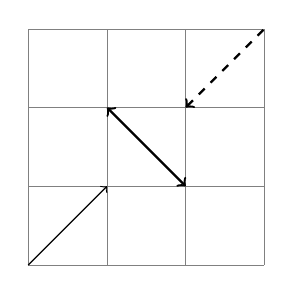
\begin{tikzpicture}
\draw[help lines] (0,0) grid (3,3);
\draw[->] (0,0) -- (1,1);
\draw[<->, thick] (2,1) -- (1,2);
\draw[<-, thick, dashed] (2,2)--(3,3);
\end{tikzpicture}
\end{frame}

\begin{frame}
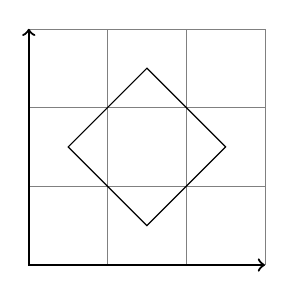
\begin{tikzpicture}
\draw[help lines] (0,0) grid (3,3);
% axes:
\draw[<->, thick] (0,3)--(0,0)--(3,0);
% diamond:
\draw (1.5,0.5) -- (2.5,1.5) --
(1.5,2.5) -- (0.5,1.5) --
cycle; % close the path
\end{tikzpicture}
\end{frame}

\begin{frame}
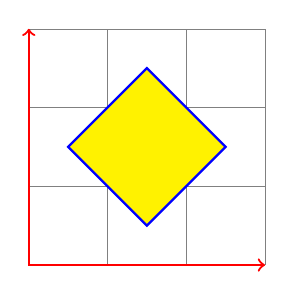
\begin{tikzpicture}
\draw[help lines] (0,0) grid (3,3);
% axes
\draw[<->, thick, red]
(0,3)--(0,0)--(3,0);
% diamond
\draw[thick, blue, fill=yellow]
(1.5,0.5) -- (2.5,1.5) --
(1.5,2.5) -- (0.5,1.5) --
cycle;
\end{tikzpicture}
\end{frame}

\begin{frame}
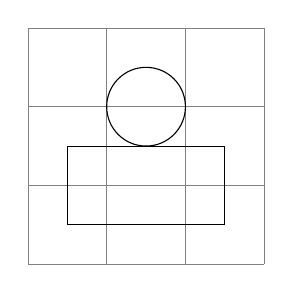
\begin{tikzpicture}
\draw[help lines] (0,0) grid (3,3);
\draw (1.5,2.0) circle (0.5);
\draw (0.5,0.5) rectangle (2.5,1.5);
\end{tikzpicture}
\end{frame}

\begin{frame}
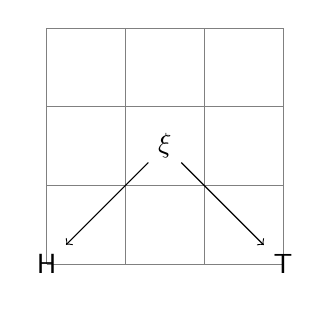
\begin{tikzpicture}
\draw[help lines] (0,0) grid (3,3);
\node (h) at (0,0) {H};
\node (x) at (1.5,1.5) {$\xi$};
\node (t) at (3,0) {T};
\draw[->] (x) -- (h);
\draw[->] (x) -- (t);
\end{tikzpicture}
\end{frame}

\begin{frame}
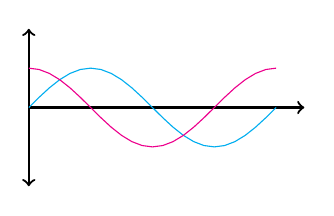
\begin{tikzpicture}[scale=0.5]
% y axis
\draw[<->, thick] (0,2) -- (0,-2);
% x axis
\draw[ ->, thick] (0,0) -- (7, 0);
% curves
\draw[cyan,domain=0:2*pi]
plot (\x, {sin(\x r)});
\draw[magenta,domain=0:2*pi]
plot (\x, {cos(\x r)});
\end{tikzpicture}
\end{frame}

\begin{frame}

\begin{tikztimingtable}
  Clock 128\,MHz 0\degr    & H   12{2C} G \\ % ends with edge
  Clock 128\,MHz 90\degr   & [C] 12{2C} C \\ % starts with edge
  Clock 128\,MHz 180\degr  & C   12{2C} G \\ % ends with edge
  Clock 128\,MHz 270\degr  &     12{2C} C \\
\end{tikztimingtable}
\begin{tikztimingtable}
  Coarse Pulse                          & 3L 16H 6L \\
  Coarse Pulse - Delayed 1              & 4L 16H 5L \\
  Coarse Pulse - Delayed 2              & 5L 16H 4L \\
  Coarse Pulse - Delayed 3              & 6L 16H 3L \\
  \\ % Gives vertical space
  Final Pulse Set                       & 3L 16H 6L \\
  Final Pulse $\overline{\mbox{Reset}}$ & 6L 16H 3L \\
  Final Pulse                           & 3L 19H 3L \\
\end{tikztimingtable}

\end{frame}

\begin{frame}
\def\degr{${}^\circ$}
\begin{tikztimingtable}
  Clock 128\,MHz 0\degr    & H 2C N(A1) 8{2C} N(A5) 3{2C} G\\
  Clock 128\,MHz 90\degr   & [C] 2{2C} N(A2) 8{2C} N(A6) 2{2C} C\\
  Clock 128\,MHz 180\degr  & C 2{2C} N(A3) 8{2C} N(A7) 2{2C} G\\
  Clock 128\,MHz 270\degr  & 3{2C} N(A4) 8{2C} N(A8) 2C C\\
  Coarse Pulse             & 3L 16H 6L \\
  Coarse Pulse - Delayed 1 & 4L N(B2) 16H N(B6) 5L \\
  Coarse Pulse - Delayed 2 & 5L N(B3) 16H N(B7) 4L \\
  Coarse Pulse - Delayed 3 & 6L 16H 3L \\
  \\
  Final Pulse Set          & 3L 16H N(B5) 6L \\
  Final Pulse $\overline{\mbox{Reset}}$ & 6L N(B4) 16H 3L \\
  Final Pulse              & 3L N(B1) 19H N(B8) 3L \\
\extracode
  \tablerules
  \begin{pgfonlayer}{background}
    \foreach \n in {1,...,8}
      \draw [help lines] (A\n) -- (B\n);
  \end{pgfonlayer}
\end{tikztimingtable}
\end{frame}

\begin{frame}
\begin{tikztimingtable}[
    timing/slope=0,         % no slope
    timing/coldist=2pt,     % column distance
    xscale=2.05,yscale=1.1, % scale diagrams
    semithick               % set line width
  ]
  \scriptsize clock     & 7{C}                              \\
  S                     & [fgblue] .75L h 2.25L H LLl       \\
  R                     & [fgblue]  1.8L .8H 2.2L 1.4H 0.8L \\
  Q                     &          L .8H 1.7L 1.5H LL       \\
  $\overline{\mbox{Q}}$ &          H .8L 1.7H 1.5L HH       \\
  Q                     & [fgred]  HLHHHLL                  \\
  $\overline{\mbox{Q}}$ & [fgred]  LHLLLHH                  \\
\extracode
 \makeatletter
 \begin{pgfonlayer}{background}
  % Draw shaded backgrounds
  \shade [right color=bgblue,left color=white]
     (7,-8.45) rectangle (-2,-4.6);
  \shade [right color=bgred,left color=white]
     (7,-12.8) rectangle (-2,-8.6);
  % Add background grid lines
  \begin{scope}[gray,semitransparent,semithick]
    \horlines{}
    \foreach \x in {1,...,6}
      \draw (\x,1) -- (\x,-12.8);
    % similar: \vertlines{1,...,6}
  \end{scope}
  % Add labels
  \node [anchor=south east,inner sep=0pt]
    at (7,-8.45) {\tiny clocked};
  \node [anchor=south east,inner sep=0pt,fgred]
    at (7,-12.8) {\tiny positive edge triggered};
 \end{pgfonlayer}
\end{tikztimingtable}%
\end{frame}

\begin{frame}
\begin{tikztimingtable}
  [timing/d/background/.style={fill=white},
   timing/lslope=0.2]
          CPOL=0 & LL 15{T} LL \\
          CPOL=1 & HH 15{T} HH \\
                 & H 17L H     \\
  \\
        Cycle \# & U     R 8{2Q} 2U    \\
            MISO & D{z}  R 8{2Q} 2D{z} \\
            MOSI & D{z}  R 8{2Q} 2D{z} \\
  \\
        Cycle \# & UU    R 8{2Q} U    \\
            MISO & D{z}U R 8{2Q} D{z} \\
            MOSI & D{z}U R 8{2Q} D{z} \\
\extracode
  % Add vertical lines in two colors
  \begin{pgfonlayer}{background}
    \begin{scope}[semitransparent,semithick]
      \vertlines[red]{2.1,4.1,...,17.1}
      \vertlines[blue]{3.1,5.1,...,17.1}
    \end{scope}
  \end{pgfonlayer}
  % Add big group labels
  \begin{scope}
    [font=\sffamily\Large,shift={(-6em,-0.5)},anchor=east]
    \node at (  0, 0) {SCK};    \node at (  0,-3 ) {SS};
    \node at (1ex,-9) {CPHA=0}; \node at (1ex,-17) {CPHA=1};
  \end{scope}
\end{tikztimingtable}%
\end{frame}


\begin{frame}
\begin{center}
\begin{tikzpicture}[node distance=2cm]
    \node (Item) [abstract, rectangle split, rectangle split parts=2]
        {
            \textbf{ITEM}
            \nodepart{second}name
        };
    \node (AuxNode01) [text width=4cm, below=of Item] {};
    \node (Component) [abstract, rectangle split, rectangle split parts=2, left=of AuxNode01]
        {
            \textbf{COMPONENT}
            \nodepart{second}nil
        };
    \node (System) [abstract, rectangle split, rectangle split parts=2, right=of AuxNode01]
        {
            \textbf{SYSTEM}
            \nodepart{second}parts
        };
    \node (AuxNode02) [text width=0.5cm, below=of Component] {};
    \node (Sensor) [abstract, rectangle split, rectangle split parts=2, left=of AuxNode02]
        {
            \textbf{SENSOR}
            \nodepart{second}nil
        };
    \node (Part) [abstract, rectangle split, rectangle split parts=2, right=of AuxNode02]
        {
            \textbf{PART}
            \nodepart{second}nil
        };
        
    \node (AuxNode03) [below=of Sensor] {};
    \node (Pressure) [abstract, rectangle split, rectangle split parts=2, left=of AuxNode03, xshift=2cm]
        {
            \textbf{Pressure}
            \nodepart{second}nil
        };
    \node (Temperature) [abstract, rectangle split, rectangle split parts=2, right=of AuxNode03, xshift=-2cm]
        {
            \textbf{Temperature}
            \nodepart{second}nil
        };
    \node (PressureInstants) [comment, rectangle split, rectangle split parts=2, below=0.2cm of Pressure, text justified]
        {
            \textbf{Instants}
            \nodepart{second}fw-p-suction\newline fw-p-delivery\newline fw-p-loop\newline sw-p-suction\newline sw-p-delivery
                \newline sw-p-loop
        };
    \node (ClOp) [abstract, rectangle split, rectangle split parts=2, below=0.4cm of PressureInstants]
        {
            \textbf{Closed/Open}
            \nodepart{second}nil
        };
    \node (ClOpInstants) [comment, rectangle split, rectangle split parts=2, below=0.2cm of ClOp, text justified]
        {
            \textbf{Instants}
            \nodepart{second}fw-clop-warm-up\newline sw-clop-control
        };
    \node (TemperatureInstants) [comment, rectangle split, rectangle split parts=2, below=0.2cm of Temperature, text justified]
        {
            \textbf{Instants}
            \nodepart{second}fw-t-engine\newline fw-t-heat-exch.\newline sw-t-heat-exch.
        };
    \node (Level) [abstract, rectangle split, rectangle split parts=2, below=0.4cm of TemperatureInstants]
        {
            \textbf{Level}
            \nodepart{second}nil
        };
    \node (LevelInstants) [comment, rectangle split, rectangle split parts=2, below=0.2cm of Level, text justified]
        {
            \textbf{Instants}
            \nodepart{second}fw-l-tank
        };
    \node (Ammeter) [abstract, rectangle split, rectangle split parts=2, below=0.4cm of LevelInstants]
        {
            \textbf{Ammeter}
            \nodepart{second}nil
        };
    \node (AmmeterInstants) [comment, rectangle split, rectangle split parts=2, below=0.2cm of Ammeter, text justified]
        {
            \textbf{Instants}
            \nodepart{second}fw-pump-ammeter\newline sw-pump-ammeter
        };
        
    \node (AuxNode04) [below=of Part] {};
    \node (Pump) [abstract, rectangle split, rectangle split parts=2, left=of AuxNode04, xshift=2cm]
        {
            \textbf{Pump}
            \nodepart{second}nil
        };
    \node (Valve) [abstract, rectangle split, rectangle split parts=2, right=of AuxNode04, xshift=-2cm]
        {
            \textbf{Valve}
            \nodepart{second}nil
        };
    \node (PumpInstants) [comment, rectangle split, rectangle split parts=2, below=0.2cm of Pump, text justified]
        {
            \textbf{Instants}
            \nodepart{second}fw-pump\newline sw-pump
        };
    \node (Tank) [abstract, rectangle split, rectangle split parts=2, below=0.4cm of PumpInstants]
        {
            \textbf{Tank}
            \nodepart{second}nil
        };
    \node (ValveInstants) [comment, rectangle split, rectangle split parts=2, below=0.2cm of Valve, text justified]
        {
            \textbf{Instants}
            \nodepart{second}fw-suction-valve\newline fw-delivery-valve\newline sw-suction-valve\newline sw-delivery-valve
                \newline sw-discharge-valve\newline sw-control-valve
        };
    \node (Engine) [abstract, rectangle split, rectangle split parts=2, below=0.4cm of ValveInstants]
        {
            \textbf{Engine}
            \nodepart{second}nil
        };
    \node (TankInstants) [comment, rectangle split, rectangle split parts=2, below=0.2cm of Tank, text justified]
        {
            \textbf{Instants}
            \nodepart{second}fw-expansion-tank
        };
    \node (HeatExchanger) [abstract, rectangle split, rectangle split parts=2, below=0.4cm of TankInstants]
        {
            \textbf{Heat Exchanger}
            \nodepart{second}nil
        };
    \node (HeatExchangerInstants) [comment, rectangle split, rectangle split parts=2, below=0.2cm of HeatExchanger, text justified]
        {
            \textbf{Instants}
            \nodepart{second}fw-heat-exchanger
        };
    \node (EngineInstants) [comment, rectangle split, rectangle split parts=2, below=0.2cm of Engine, text justified]
        {
            \textbf{Instants}
            \nodepart{second}fw-engine
        };
    \node (Strainer) [abstract, rectangle split, rectangle split parts=2, below=0.4cm of HeatExchangerInstants]
        {
            \textbf{Strainer}
            \nodepart{second}nil
        };
    \node (StrainerInstants) [comment, rectangle split, rectangle split parts=2, below=0.2cm of Strainer, text justified]
        {
            \textbf{Instants}
            \nodepart{second}sw-strainer
        };
    \node (Coolant) [abstract, rectangle split, rectangle split parts=2, below=0.4cm of EngineInstants]
        {
            \textbf{Coolant}
            \nodepart{second}nil
        };
    \node (CoolantInstants) [comment, rectangle split, rectangle split parts=2, below=0.2cm of Coolant, text justified]
        {
            \textbf{Instants}
            \nodepart{second}fw-coolant\newline sw-coolant
        };  

    \node (AuxNode05) [below=of System] {};
    \node (CoolingSystem) [abstract, rectangle split, rectangle split parts=2, left=of AuxNode05, xshift=2cm]
        {
            \textbf{Cooling System}
            \nodepart{second}nil
        };
    \node (CoolingLoop) [abstract, rectangle split, rectangle split parts=2, right=of AuxNode05, xshift=-2cm]
        {
            \textbf{Cooling Loop}
            \nodepart{second}nil
        };
    \node (CoolingSystemInstants) [comment, rectangle split, rectangle split parts=2, below=0.2cm of CoolingSystem, text justified]
        {
            \textbf{Instants}
            \nodepart{second}cool
        };
    \node (CoolingLoopInstants) [comment, rectangle split, rectangle split parts=2, below=0.2cm of CoolingLoop, text justified]
        {
            \textbf{Instants}
            \nodepart{second}fw-loop\newline sw-loop
        };
    
    \draw[myarrow] (Component.north) -- ++(0,0.8) -| (Item.south);
    \draw[line] (Component.north) -- ++(0,0.8) -| (System.north);
    
    \draw[myarrow] (Sensor.north) -- ++(0,0.8) -| (Component.south);
    \draw[line] (Sensor.north) -- ++(0,0.8) -| (Part.north);
    
    \draw[line] (Pressure.west) -- ++(-0.2,0);
    \draw[line] (Temperature.east) -- ++(0.2,0);
    \draw[line] (Level.east) -- ++(0.2,0);
    \draw[myarrow] (ClOp.west) -- ++(-0.2,0) -- ([yshift=0.5cm, xshift=-0.2cm] Pressure.north west) -|
     ([xshift=-1cm]Sensor.south);
    \draw[myarrow] (Ammeter.east) -- ++(0.2,0) -- ([yshift=0.5cm, xshift=0.2cm] Temperature.north east) -|
     ([xshift=1cm]Sensor.south);
     
    \draw[line] (Tank.west) -- ++(-0.2,0);
    \draw[line] (HeatExchanger.west) -- ++(-0.2,0);
    \draw[line] (Pump.west) -- ++(-0.2,0);
    \draw[line] (Valve.east) -- ++(0.2,0);
    \draw[line] (Engine.east) -- ++(0.2,0);
    \draw[myarrow] (Strainer.west) -- ++(-0.2,0) -- ([yshift=0.5cm, xshift=-0.2cm] Pump.north west) -|
     ([xshift=-1cm]Part.south);
    \draw[myarrow] (Coolant.east) -- ++(0.2,0) -- ([yshift=0.5cm, xshift=0.2cm] Valve.north east) -|
     ([xshift=1cm]Part.south);
     
    \draw[myarrow] (CoolingSystem.north) -- ++(0,0.8) -| (System.south);
    \draw[line] (CoolingSystem.north) -- ++(0,0.8) -| (CoolingLoop.north);
        
        
\end{tikzpicture}
\end{center}
\end{frame}

\begin{frame}
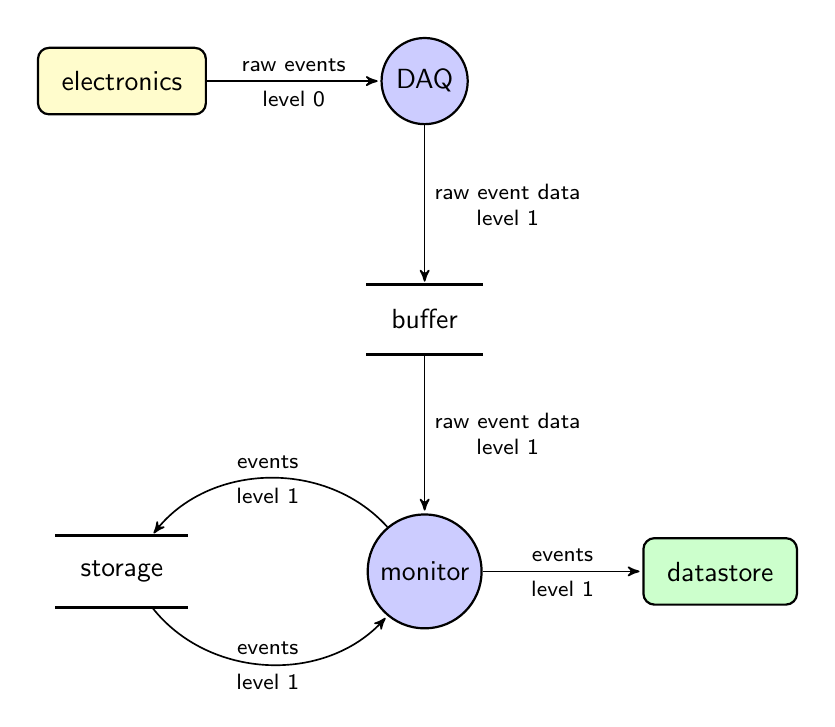
\begin{tikzpicture}[
  font=\sffamily,
  every matrix/.style={ampersand replacement=\&,column sep=2cm,row sep=2cm},
  source/.style={draw,thick,rounded corners,fill=yellow!20,inner sep=.3cm},
  process/.style={draw,thick,circle,fill=blue!20},
  sink/.style={source,fill=green!20},
  datastore/.style={draw,very thick,shape=datastore,inner sep=.3cm},
  dots/.style={gray,scale=2},
  to/.style={->,>=stealth',shorten >=1pt,semithick,font=\sffamily\footnotesize},
  every node/.style={align=center}]

  % Position the nodes using a matrix layout
  \matrix{
    \node[source] (hisparcbox) {electronics};
      \& \node[process] (daq) {DAQ}; \& \\

    \& \node[datastore] (buffer) {buffer}; \& \\

    \node[datastore] (storage) {storage};
      \& \node[process] (monitor) {monitor};
      \& \node[sink] (datastore) {datastore}; \\
  };

  % Draw the arrows between the nodes and label them.
  \draw[to] (hisparcbox) -- node[midway,above] {raw events}
      node[midway,below] {level 0} (daq);
  \draw[to] (daq) -- node[midway,right] {raw event data\\level 1} (buffer);
  \draw[to] (buffer) --
      node[midway,right] {raw event data\\level 1} (monitor);
  \draw[to] (monitor) to[bend right=50] node[midway,above] {events}
      node[midway,below] {level 1} (storage);
  \draw[to] (storage) to[bend right=50] node[midway,above] {events}
      node[midway,below] {level 1} (monitor);
  \draw[to] (monitor) -- node[midway,above] {events}
      node[midway,below] {level 1} (datastore);
\end{tikzpicture}
\end{frame}

\begin{frame}
\begin{tikzpicture}[%
  grow via three points={one child at (0.5,-0.7) and
  two children at (0.5,-0.7) and (0.5,-1.4)},
  edge from parent path={(\tikzparentnode.south) |- (\tikzchildnode.west)}]
  \node {texmf}
    child { node {doc}}     
    child { node {fonts}}
    child { node {source}}
    child { node [selected] {tex}
      child { node {generic}}
      child { node [optional] {latex}}
      child { node {plain}}
    }
    child [missing] {}              
    child [missing] {}              
    child [missing] {}              
    child { node {texdoc}};
\end{tikzpicture}
\end{frame}

\begin{frame}
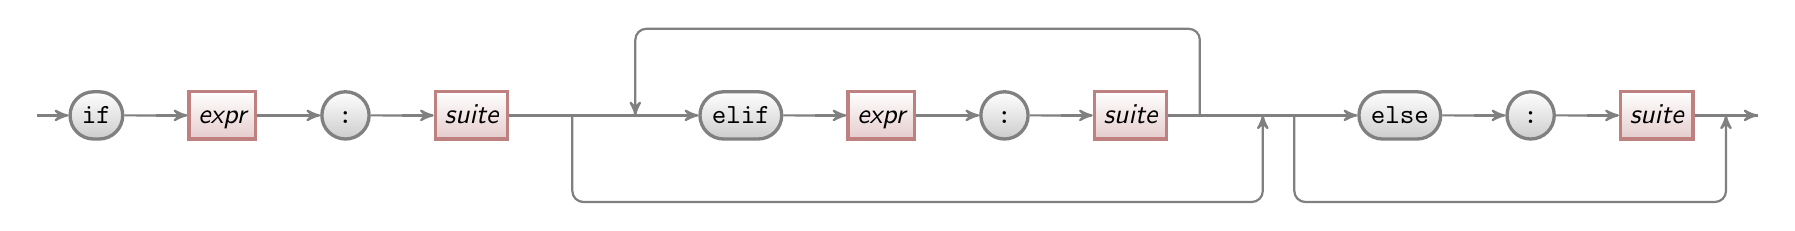
\begin{tikzpicture}[point/.style={coordinate},>=stealth',thick,draw=black!50,
                    tip/.style={->,shorten >=0.007pt},every join/.style={rounded corners},
                    hv path/.style={to path={-| (\tikztotarget)}},
                    vh path/.style={to path={|- (\tikztotarget)}},
                    text height=1.5ex,text depth=.25ex]     % um die Hoehe des Punktes festzuzurren
  \matrix[ampersand replacement=\&,column sep=4mm] {
    \node (p1)  [point]  {}; \&    \node (ifs)    [terminal]     {if};             \&
    \node (p2)  [point]  {}; \&    \node (expr1)  [nonterminal]  {expr};           \&
    \node (p3)  [point]  {}; \&    \node (colon1) [terminal]     {:};              \&
    \node (p4)  [point]  {}; \&    \node (suite1) [nonterminal]  {suite};          \&
    \node (p5)  [point]  {}; \&    \node (p6)     [point]  {};                     \&
    \node (p6a) [point]  {}; \&    \node (p6b)    [point]  {};                     \&
    \node (p7)  [point]  {}; \&    \node (elif)   [terminal]     {elif};           \&
    \node (p8)  [point]  {}; \&    \node (expr2)  [nonterminal]  {expr};           \&
    \node (p9)  [point]  {}; \&    \node (colon2) [terminal]     {:};              \&
    \node (p10) [point]  {}; \&    \node (suite2) [nonterminal]  {suite};          \&
    \node (p11) [point]  {}; \&    \node (p12)    [point]  {};                     \&
    \node (p12a)[point]  {}; \&    \node (p12b)   [point]  {};                     \&
    \node (p13) [point]  {}; \&    \node (else)   [terminal]     {else};           \&
    \node (p14) [point]  {}; \&    \node (colon3) [terminal]     {:};              \&
    \node (p15) [point]  {}; \&    \node (suite3) [nonterminal]  {suite};          \&
    \node (p16) [point]  {}; \&    \node (p17)    [point]       {};\\
  };

  { [start chain]
    \chainin (p1);
    \chainin (ifs)    [join=by tip];
    \chainin (p2)     [join];
    \chainin (expr1)  [join=by tip];
    \chainin (p3)     [join];
    \chainin (colon1) [join=by tip];
    \chainin (p4)     [join];
    \chainin (suite1) [join=by tip];
    \chainin (p7)     [join];
    \chainin (elif)   [join=by tip];
    \chainin (p8)     [join];
    \chainin (expr2)  [join=by tip];
    \chainin (p9)     [join];
    \chainin (colon2) [join=by tip];
    \chainin (p10)    [join];
    \chainin (suite2) [join=by tip];
    \chainin (p12a)   [join,join=with p6 by {skip loop=-11mm,tip}];
    \chainin (p13)    [join];
    \chainin (else)   [join=by tip];
    \chainin (p14)    [join];
    \chainin (colon3) [join=by tip];
    \chainin (p15)    [join];
    \chainin (suite3) [join=by tip];
    \chainin (p16)    [join];
    \chainin (p17)    [join=by tip];
    \chainin (p16)    [join,join=with p12b by {skip loop=-11mm,tip}];
    \chainin (p6b)    [join=with p11 by {skip loop=11mm,tip}];
  }
\end{tikzpicture}
\end{frame}

\begin{frame}
\begin{wave}{13}{5}
 \nextwave{req\_addr} \bit{0}{.2} \bit{1}{1} \bit{0}{3} \bit{1}{1} \bit{0}{.8}
 \nextwave{inst\_addr} \unknown[X]{.5} \known{addr}{1} \unknown{4.5}
 \nextwave{link\_addrs} \unknown{1.2} \known{map}{1} \unknown{3.8}
 \nextwave{link\_load} \unknown{2.2} \known{vam}{1} \unknown{2.8}
 \nextwave{link\_load\_r} \unknown{3.1} \known{val}{1} \unknown{1.9}
 \nextwave{simulate} \bit{0}{3.1} \bit{1}{1} \bit{0}{1.9}
 \nextwave{output} \unknown{3.3} \known{}{.5} \known{}{.5} \unknown{1.7}
 \nextwave{prev\_output} \unknown{3.2} \known{old}{1} \unknown{1.8}
 \nextwave{differs} \unknownbit{3.3} \bit{1}{.5} \bit{1}{.4} \unknownbit{1.8}
 \nextwave{differs\_r} \unknownbit{4.1} \bit{1}{1} \unknownbit{.9}
 \nextwave{dep\_addr} \unknown{4.2} \known{dep}{1} \unknown[X]{.8}
 \nextwave{req} \unknown{4.3} \known{req}{1} \unknown[X]{.7}
\end{wave}
\end{frame}

\begin{frame}
  \begin{tikztimingtable}
    {CLK} & 30{C} \\
    {$\overline{RESETn}$} & 2{H}10{L}18{H} \\
    {$\overline{NCE}$}    & 14{H}4{L}12{H} \\
  \end{tikztimingtable}

  \begin {tikztimingtable}
    Name & hLLLLh \\
    Clock & 10{ c } \\
    Signal & z4D { Text } z \\
  \end {tikztimingtable}
\end{frame}

\end{document}